\section*{Data Sources, Modeling choices}

We use the LFM with $k=2$ on the two aforementioned measures of state amity to generate a combined measure of state preference similarity which accounts for network effects. As inputs, we use the UN voting similarity index \citep{voeten:2013}\footnote{Specifically, the ``agree3un'' variable.} and number of alliance relationships between states by time $t$ \citep{gibler:sarkees:2004}. However, to facilitate comparison between the metrics, we first standardize and normalize these two measures. This gives us an $n \times n \times T \times 2$ array, where the first two dimensions represent countries, the third dimension is the year, and the fourth is the particular measure of similarity. So the item at index (1,2,1,1) would be the transformed value of the S-score for countries $i$ and $j$ at the first year of our data, similarly (1,2,1,2) would be the UN ideal point distance measure.

% Another important question is the amount of temporal aggregation used. In our baseline model, we treat each year as separate and gain a unique observation of each states ideal point in each year. However, this raises a real risk of temporal inconsistency in the values. An alternative approach would be to have a rolling average for the measures of similarity over a number of years. This would allow us to infer a country's relative position not just by their behavior in a given year, but also their behavior in the past few years. The risk if we use too much temporal aggregation is that we are including data which is no longer relevant to a country's relative preferences. For instance, Turkey and Russia's relationship looks a lot more positive when we look at 2013 and 2014 then when we look at 2015. To that end, in addition to our baseline model where years are seen as independent, we also evaluate models where ... 

With this data, we run an LFM with a Gaussian link, and in particular we use the $U \Lambda U^{\top}$ term produced by each yearly model to estimate each states position in a two-dimensional hypersphere. We then evaluate whether their is additional utility gained from using this latent angle position, as compared to the similarity of alliance portfolios and UN ideal point distance measures.

\subsection*{Face Plausibility}

An important question for these different measures of preferences, are whether they give results that ``make sense" for prominent pairs of countries. In particular we would hope that the measure both provides plausible levels to relationships -- sorting states into friends and foes effectively -- and that when these measures change, they do so in ways that correspond to changes in the world. We thus present all three measures' accounts of eight dyadic relationships over time.\footnote{For the sake of having each measure operate in the same direction, we transform the S-score such that the value shown is 1 - S. Thus for all three variables, $0$ implies perfect symmetry of preferences.} Additionally, note that each of these measures is on a different scale, and so just because one measure has a higher value, does not necessarily mean that it posits more dissimilarity of preferences.

We first look at three close relationships where we would expect to see similar preferences. Figure \ref{friendly:dyads} depicts the relationships between France and Germany, the US and Israel, and North Korea and China. In all three cases our measure using latent angle distance has consistently low values -- nearly $0$ in the case of France and Germany, and China and North Korea, and low but less stable values for the US/Israel relationship. Alliance S-Scores correctly classifies Franco-German and Sino-North Korean friendship, while the US/Israel relationship is characterized as being relatively neutral. The measure based on UN voting is most out of step in terms of characterizing these relationships, with notable divergence in the preferences of many of these pairs.

\begin{figure}
	\centering
	\includegraphics[width=1\textwidth]{plausPlot_1}
	\caption{Dyadic relationships between 3 pairs of countries according to the different preference measures. Yearly latent angle distances between dyads are denoted by red circles and ideal point distance based on UN voting in blue triangles. S-score values have been rescaled such that they works in the same direction as the other measures (1-S-score, so that the best score is 0), and are depicted by green squares.}
	\label{friendly:dyads}
\end{figure}

In figure \ref{unfriendly:dyads} we look at the United States' relationship with three countries that are characterized by change and major events. S-scores are the only measure that does not detect a marked improvement in the US/Russian relationship at the end of the Cold War. Both the UN ideal points and latent Angle space find significant improvements followed by a drift toward enmity, whereas S-scores have a constant (though slightly improving) neutral relationship. For the US and Iraq no measure depicts more similar preferences following the US occupation, though only latent angle distance finds an increase in enmity in the run-up to the United States' invasion. Finally, for the US and China, the S-score has a consistent neutral relationship, while both UN ideal points and latent angles both have more negative relationships, and more variance -- with the latent angles metric finding particularly large spikes at the beginning of the Bush and Obama administrations.

\begin{figure}
	\centering
	\includegraphics[width=1\textwidth]{plausPlot_2}
	\caption{Dyadic relationships between 3 pairs of countries according to the different preference measures. Yearly latent angle distances between dyads are denoted by red circles and ideal point distance based on UN voting in blue triangles. S-score values have been rescaled such that they works in the same direction as the other measures (1-S-score, so that the best score is 0), and are depicted by green squares.}
	\label{unfriendly:dyads}
\end{figure}

A big difference between these measures is that latent angle distance has a fuller time series than the other two. This is particularly relevant when looking at the preferences of certain rogue states, as we do in figure \ref{missing:dyads}. In both the case of Iran/Iraq and North Korea/South Korea there is no data for UN voting (and for Iran/Iraq missing data for S-scores). For the Korean relationship, latent angle distance better characterizes the relationship as enmity, while S-scores treat the two as having very similar preferences. Whereas for Iran and Iraq's relationship S-scores give a consistent close preferences (where data exists), while the latent angle metric show more instability, and notable elevation (though not as large as we would expect) during their war.


\begin{figure}
	\centering
	\includegraphics[width=.67\textwidth]{plausPlot_3}
	\caption{Dyadic relationships between 2 pairs of countries according to the different preference measures. Yearly latent angle distances between dyads are denoted by red circles and ideal point distance based on UN voting in blue triangles. S-score values have been rescaled such that they works in the same direction as the other measures (1-S-score, so that the best score is 0), and are depicted by green squares.}
	\label{missing:dyads}
\end{figure}

As can be seen from these relationships, the measure of preferences based on latent angle distance is in many cases as plausible or more than incumbent measures of preferences. While the measure has more temporal instability than S-scores or UN ideal points, in these 8 cases it often does better, and rarely worse at conforming to our expectations of the relationships. Of course, this could just be a case of us picking particularly propitious cases. Next, we conduct a the large-N analysis of conflict and compare the added utility of these various measures of state preferences.

\subsection*{Model Competition}

To evaluate the different measures of state preferences, we assess their utility in predicting the occurrence of interstate disputes. Here we look at four non-nested models: a model using no measures of state preferences, one using an S-Score based on similarity in alliance portfolio \citep{signorino:ritter:1999}, one using the ideal points determined by UN voting \citep{bailey:etal:2015}, a model using both UN ideal points and alliance S-scores, and finally, a model using our latent angle approach to combine data from UN voting and alliances. We evaluate the models on two criteria: whether state preferences have a consistent effect in the predicted direction, and how well each model does at predicting disputes on out of sample data.

In each of these models, we utilize a logistic regression of Militarized Interstate Dispute (MID) participation on measures of state preferences and a vector of control variables. These control variables overlap with the standard framework used in O'Neal and Russett's canonical work on the democratic peace \citep{oneal:russett:1997}.\footnote{The exception is that our models ignore trade interdependency, as including that data drastically decreases the number of observations.} In particular, we include a binary measure of joint democracy (whether both states have Polity IV scores $geq 7$), whether the states are contiguous, and the ratio of state capabilities as measured by the Correlates of War Project's Composite Index of National Capabilities (CINC). We also account for temporal interdependence using a peace year spline \citep{carter:signorino:2010}. 

\subsection*{In sample explanation}

As detailed in figure \ref{fig:coefP}, each measure of state preferences behaves as we would expect. Our measure of state preference using latent angle difference is highly significant and positive: states with more dissimilar preferences will have greater difference in their latent angles, and this is highly associated with a greater risk of conflict. Similarly, both incumbent measures of preferences pass this test. The measure using UN voting ideal points is positive and clearly distinct from $0$, indicating that states with more distant ideal points, and thus more dissimilar preferences, are more likely to find themselves in conflict. Similarly, higher alliance S-scores are consistently associated with lower probabilities of conflict -- so states with more similar preferences as measured using alliance portfolios are less likely to quarrel. These results hold when those measures of preference are used in isolation, or in tandem.

The models have one major difference in terms of the controls: in the model using latent angle distance, joint democracy is indistinguishable from $0$. This is particularly interesting as one of the major criticisms of democratic peace theory is that democracies have similar preferences. Some argue that it is similarity in preferences that leads to peace among democracies.  Despite this dispute, most attempts to include preferences in the standard democratic peace regressions still find a consistent pacifying effect of democracy.
(as do those models with UN voting and S-scores presented here). With our measure of preferences, however, democracy's effect is negligible. More research is necessary to disentangle whether the criticism is now credible, but work such as this provides a template for us to parse out the effect of democracy versus preferences on conflict.


\begin{figure}[ht]
	\centering
	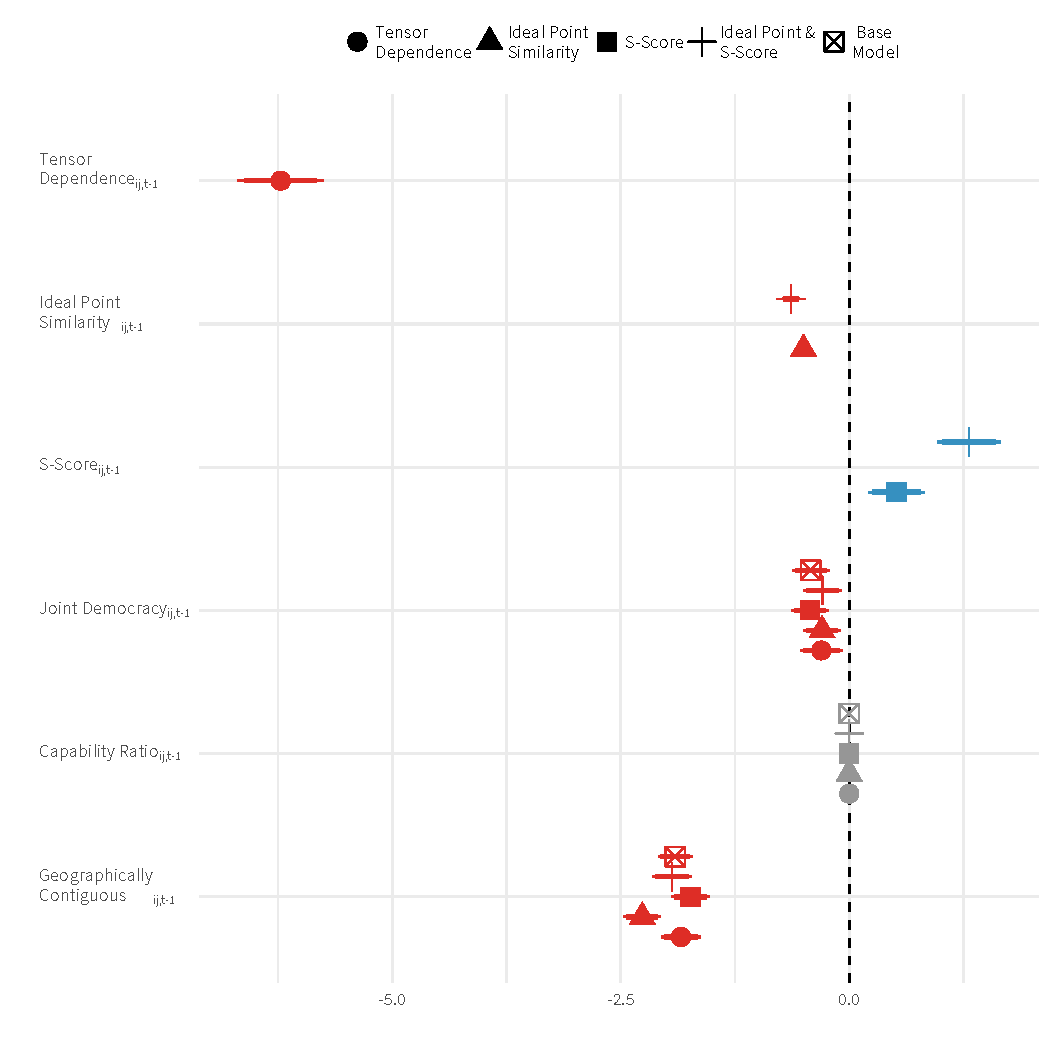
\includegraphics[width=.7\textwidth]{betaEst}
	\caption{Parameter estimates from models with different measures of state preference. Point represents average estimate, line through the point represents the 95\% confidence interval.}
	\label{fig:coefP}
\end{figure}
\FloatBarrier

\subsection*{Out-of-sample prediction}

Given these results, we can say that all of the measures of preferences behave as we would expect. To adjudicate which measures best capture state preferences, and what we should make of the differing effect of democracy, we turn to out of sample prediction. We undertake a cross-validation procedure in which we partition our data into 30 different folds. This process works by taking each fold, $k$, and running a logistic model excluding data from that fold. Once we have parameter estimates from a model that excluded fold $k$, we predict the probability of a MID in fold $k$ using only the parameter estimates and the covariates from fold $k$.

We then compare the performance of these models using the area under both the Receiver Operator Characteristic Curve (AUC ROC) and under the Precision Recall Curve (AUC PR). The AUC ROC curve examines the tradeoff between true positives and false positives, and the AUC PR examines the tradeoff between making only correct predictions and predicting all the disputes that occurred. In general, the AUC ROC will disproportionately reward those models that predict $0$ well -- and we can interpret the AUC ROC as the likelihood a prediction is correct. The numeric value for the AUC PR has less of a clear interpretation, but models with a higher AUC PR do a better job of predicting when events actually occur.

As shown in figure \ref{fig:roc}, the model using latent angle distance decisively outperforms all the other models. While the AUC ROC is somewhat higher with the latent Angle model, the real difference between the measures shines through in the AUC PR, where the model using this measure performs twice as well as the base model. In contrast, models using other measures of state preferences yield only minimal improvements in prediction over the base model. This is especially relevant because AUC PR specifically focuses on the difficult task of predicting conflict, compared to the relatively easier task of predicting non-conflict that is rewarded by the AUC ROC measure. Thus we have reason for confidence in both the usefulness of this measure of state preferences and renewed reason for skepticism in the effect of joint democracy once we control for state preferences. 

\begin{figure}[ht]
	\centering
	\begin{tabular}{cc}
	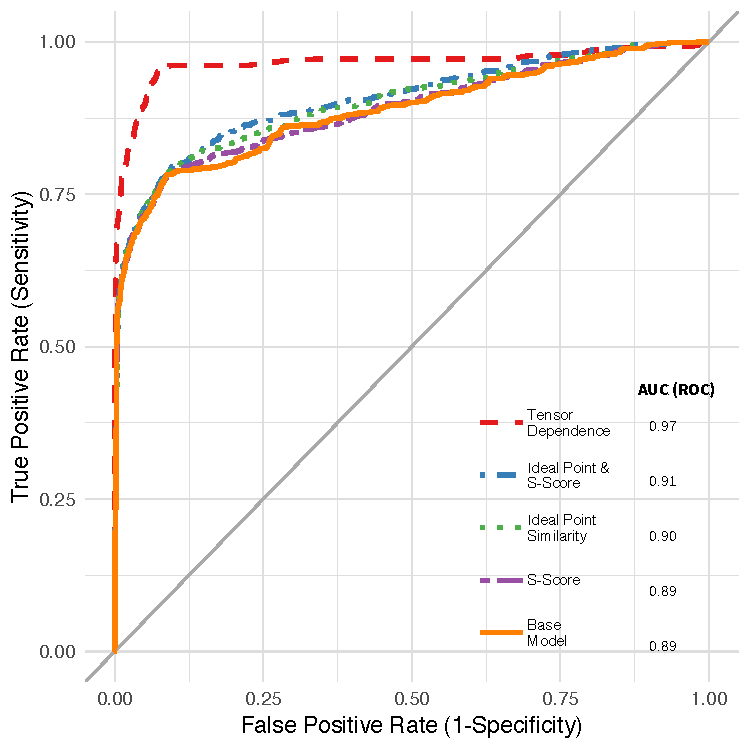
\includegraphics[width=.5\textwidth]{roc_outSample} & 
	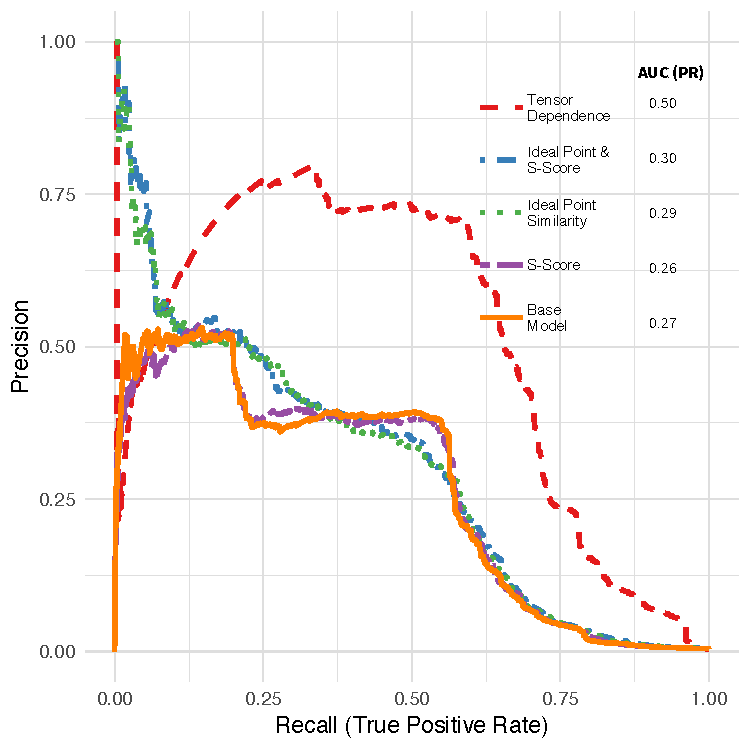
\includegraphics[width=.5\textwidth]{rocPr_outSample}	
	\end{tabular}
	\caption{Assessments of out-of-sample predictive performance using ROC curves and PR curves. AUC statistics are provided as well for both curves.}
	\label{fig:roc}
\end{figure}
\FloatBarrier
